\chapter{Numerical issues}

The numerical implementation of the Casimir effect in the plane--sphere
geometry is a challenging task. The main problem is the competing demands on
the numerical implementation: stability and performance. On the one hand, the
code has to be stable over a wide range of parameters. On the other hand, the
implementation is supposed to be fast in order to obtain results in a bearable
time.

Luckily, we do not have to reinvent the wheel, but we may profit from the
experience of \textsc{Canaguier--Durand} \cite{Durand}. In this chapter, we will
focus on the problems that are either not covered by \textsc{Canaguier--Durand}
or that we have solved in a different way.

\section{Truncation of the vector space}

\begin{figure}
    \begin{minipage}[b]{.5\linewidth}
    \centering
    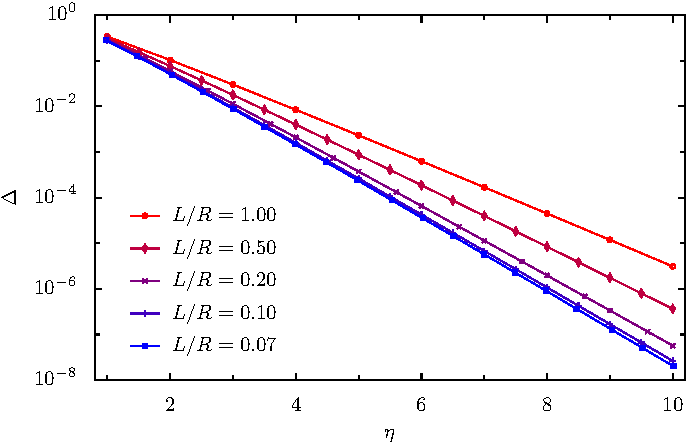
\includegraphics[scale=0.66]{plots/numeric/convergence_lmax/convergence_0_50.pdf}
    \subcaption{$T=0.5$}
    \end{minipage}%
    \begin{minipage}[b]{.5\linewidth}
    \centering
    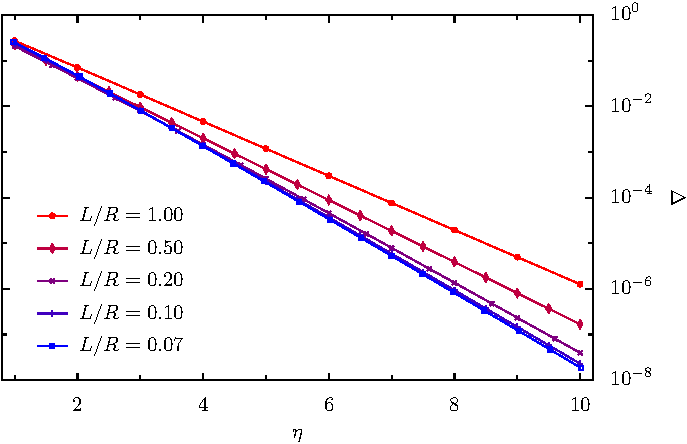
\includegraphics[scale=0.66]{plots/numeric/convergence_lmax/convergence_10_00.pdf}
    \subcaption{$T=10$}
    \end{minipage}

  \caption{Accuracy of the free energy as a function of the coefficient $\eta$. We show the achieved
  accuracy for several separations $L/R$ for a) $T=0.5$ and b) $T=10$. ($\eta_\text{c}=20$)}
  \label{fig:convergence_lmax}
\end{figure}

For the implementation one has to truncate the dimension of the scattering
matrix $\mathcal{D}$ to a finite value. This means that we only take
multipole waves up to a moment $\lmax$ into account. As the scattering
matrix consists of four block matrices, its dimension is thus
$2\lmax\times2\lmax$.

From a physical point of view it is reasonable that for values of
$\ell_\text{max}$ sufficiently large the value of the free energy converges.
This is argued qualitatively in Ref. \cite{Durand}. It turns out that for
smaller separations more multipole moments are needed in order to obtain the
same accuracy. For this reason, we define a coefficient $\eta$ and determine
$\ell_\text{max}$ by
\begin{equation}
\ell_\text{max} = \left\lceil \eta \frac{R}{L} \right\rceil .
\end{equation}
Fig. \ref{fig:convergence_lmax} shows the dependence of the accuracy on
$\eta$. The accuracy is defined by
\begin{equation}
\Delta = \left| \frac{\mathcal{F}(\eta)-\mathcal{F}(\eta\to\infty)}{\mathcal{F}(\eta\to\infty)} \right|
 \approx \left| \frac{\mathcal{F}(\eta)-\mathcal{F}(\eta_\text{c})}{\mathcal{F}(\eta_\text{c})} \right| \\
 \text{for} \sep \eta_\text{c} \gg \eta,
\end{equation}
and corresponds to the deviation from the exact result. Fig.
\ref{fig:convergence_lmax} reveals that the accuracy $\Delta$ depends
exponentially on $\eta$. Also, the accuracy depends only weakly on the
temperature and for a chosen value of $\eta$ the accuracy becomes better for
smaller separations. To obtain an accuracy of $10^{-4}$ one has to choose
$\eta\approx6$ for separations $L/R \lesssim 0.2$.


\section{Modified Bessel functions and Mie coefficients}

The definition of the Mie coefficients $a_\ell$, $b_\ell$ involves modified
Bessel functions of the first $I_\nu(x)$ and of the second kind $K_\nu(x)$.  We
briefly outline the ideas of \textsc{Canaguier--Durand} \cite{Durand}.  The
modified Bessel functions for half-integer indices obey for $\ell > 2$ the
recurrence relations (cf. \eqref{eq_appendix_bessel_recurrence})
\begin{equation}
\label{numerics_bessel_recurrence}
I_{\ell+\frac{1}{2}}(x) = I_{\ell-\frac{3}{2}}(x) - \frac{(2\ell-1)I_{\ell-\frac{1}{2}}(x)}{x}, \\
K_{\ell+\frac{1}{2}}(x) = K_{\ell-\frac{3}{2}}(x) + \frac{(2\ell-1)K_{\ell-\frac{1}{2}}(x)}{x}.
\end{equation}
With the initial functions
\begin{align}
\label{numerics_bessel_start}
I_{\frac{1}{2}}(x) &= \sqrt{\frac{2}{\pi x}} \sinh x,   & I_{\frac{3}{2}} &= \sqrt{\frac{2}{\pi x}}\left(\cosh x - \frac{\sinh x}{x}\right), \\
K_{\frac{1}{2}}(x) &= \sqrt{\frac{\pi}{2 x}} \e^{-x},   & K_{\frac{3}{2}} &= \sqrt{\frac{\pi}{2x}} \left(1 + \frac{1}{x}\right) \e^{-x},
\end{align}
the recurrence relations can be exploited to calculate the modified Bessel
functions. This procedure works fine for $K_{\ell+\frac{1}{2}}(x)$, however, it
is unstable for $I_{\ell+\frac{1}{2}}(x)$. The subtraction of two almost
identical numbers is numerically ill-conditioned and causes a loss of
significance. The recurrence formula for $I_{\ell+\frac{1}{2}}(x)$ contains
such a subtraction which renders this method impractical for calculating
$I_{\ell+\frac{1}{2}}(x)$.

The function $I_{\ell+\frac{1}{2}}(x)$ can be computed by a downward recurrence
relation
\begin{equation}
\label{numerical_bessel_cfrac}
I_{\ell+\frac{1}{2}}(x) = \frac{1}{x} \left(K_{\ell+\frac{3}{2}}(x) + f_{\ell+\frac{1}{2}}(x) K_{\ell+\frac{1}{2}}(x)\right)^{-1},
\end{equation}
where
\begin{equation}
f_{\ell+\frac{1}{2}}(x) = \frac{I_{\ell+\frac{3}{2}}(x)}{I_{\ell+\frac{1}{2}}(x)} = \frac{1}{\frac{2(\ell+1)+1}{x} + \frac{1}{\frac{2(\ell+2)+1}{x} + \dots}} = [a_1, a_2, a_3, \dots]
\end{equation}
is a continued fraction with coefficients
\begin{equation}
a_n = \frac{2(\ell+n)+1}{x}.
\end{equation}
Eq. \eqref{numerical_bessel_cfrac} has the disadvantage that the accuracy of
$f_{\ell+\frac{1}{2}}$ cannot be improved in an iterative way: if the accuracy
is unsatisfactory the calculation has to be repeated from the beginning.
However, $f_{\ell+\frac{1}{2}}$ can be modified to
\begin{equation}
\label{eq:numerics_bessel_cfrac}
f^N_{\ell+\frac{1}{2}}(x) = [a_1, a_2, \dots, a_N] = \frac{[a_1] \cdot [a_2,a_1] \cdot \, \dots \, \cdot [a_N,\dots,a_2,a_1]}{[a_2] \cdot [a_3,a_2] \cdot \, \dots \, \cdot [a_N, \dots, a_3, a_2]}
\end{equation}
and the continued fraction can be computed up to the desired accuracy.

Given the modified Bessel functions, it is easy to compute the Mie
coefficients. The Mie coefficients are evaluated at the argument $\chi =
nTR/\mathcal{L}$ which only depends on $n$. For a given value of $n>0$ it is
thus sufficient to compute the Mie coefficients $a_1, \dots, a_\lmax$ and $b_1,
\dots, b_\lmax$ once and store the results. For this reason, the time needed to
calculate the Mie coefficients is negligible compared to the total computational time.

\section{Integration}

For the numerical evaluation of the integrals we first perform a change of variable.
We substitute
\begin{equation}
z = \frac{2\kappa}{\tau}-1, \\ k = \frac{\tau}{2}\sqrt{z^2+2z}, \\ \kappa = \frac{\tau}{2} \left(z+1\right), \\ \mathrm{d}z = \frac{2k}{\tau\kappa} \mathrm{d}k,
\end{equation}
and obtain
\begin{align}
\label{numerical_intA}
A_{\ell_1\ell_2,p}^{(m)} &= (-1)^{\ell_2+m} \, m^2 \, \e^{-\tau} \int_0^\infty \mathrm{d}z \, \frac{r_p \, \e^{-\tau z}}{z^2+2z} \, \Plm{\ell_1}{m}\left(1+z\right) \Plm{\ell_2}{m}\left(1+z\right), \\
\label{numerical_intB}
B_{\ell_1\ell_2,p}^{(m)} &= (-1)^{\ell_2+m+1} \, \e^{-\tau} \int_0^\infty \mathrm{d}z \, r_p \, \e^{-\tau z} \, (z^2+2z) \, \Plm{\ell_1}{m}^\prime\left(1+z\right) \Plm{\ell_2}{m}^\prime\left(1+z\right), \\
\label{numerical_intC}
C_{\ell_1\ell_2,p}^{(m)} &= \imag m (-1)^{\ell_2+m} \, \e^{-\tau} \int_0^\infty \mathrm{d}z \, r_p \, \e^{-\tau z} \, \Plm{\ell_1}{m}\left(1+z\right) \Plm{\ell_2}{m}^\prime\left(1+z\right), \\
\label{numerical_intD}
D_{\ell_1\ell_2,p}^{(m)} &= (-1)^{\ell_1+\ell_2+1} C_{\ell_2\ell_1,p}^{(m)}
\end{align}
where we have introduced the abbrevation $\tau \equiv 2nT$ and used the parity
of the associated Legendre polynomials (cf.
\eqref{appendix_sfun_assoclegendre_parity}).
One way to solve the integrals \eqref{numerical_intA}--\eqref{numerical_intD} numerically is to use Gauss-Laguerre quadrature.
For perfect reflectors the Fresnell coefficients $r_p$ are mere numbers and can be put in front of the integral. The integrand
is then of the form of a polynomial times a decreasing exponential function. For this reason Gauss-Laguerre integration becomes
exact if the order is sufficiently high.

However, we will follow a different way here. The product of two associated
Legendre polynomials can be expressed as a sum of associated Legendre polynomials
\begin{equation}
\Plm{n}{m}(x) \Plm{\nu}{\mu}(x) = a_0 \sum_{q=0}^\qmax \tilde a_q  \Plm{n+\nu-2q}{m+\mu}(x),
\end{equation}
where the prefactor $a_0$ and the Gaunt coefficients $\tilde a_q$ are defined in \cite{Xu199753}. Using
Gaunt coefficients, each integral \eqref{numerical_intA}--\eqref{numerical_intD} can
be reduced to a sum of integrals of the type
\begin{equation}
\mathcal{J}_\nu^{2m}(\tau) = \int_0^\infty \mathrm{d}z \, \frac{\e^{-\tau x}}{z^2+2z} \Plm{\nu}{2m}\left(1+z\right).
\end{equation}
For $A_{\ell_1\ell_2,p}^{(m)}(\tau)$ we find
\begin{align}
\nonumber
A_{\ell_1\ell_2,p}^{(m)}(\tau) &= \overbrace{(-1)^{\ell_2+m} \, r_p \, m^2 \, \e^{-\tau}}^{\equiv A_0} \int_0^\infty \mathrm{d}z \, \frac{\e^{-\tau z}}{z^2+2z} \, \Plm{\ell_1}{m}(1+z) \Plm{\ell_2}{m}(1+z) \\
&= A_0 \, a_0 \sum_{q=0}^\qmax \tilde a_q \int_0^\infty \mathrm{d}z \, \frac{\e^{-\tau z}}{z^2+2z} \, \Plm{\ell_1+\ell_2-2q}{2m}(1+z) = A_0 \, a_0 \sum_{q=0}^\qmax \tilde a_q \, \mathcal{J}_{\ell_1+\ell_2-2q}^{2m}(\tau),
\end{align}
for $B_{\ell_1\ell_2,p}^{(m)}(\tau)$
\begin{align}
\nonumber
&B_{\ell_1\ell_2,p}^{(m)}(\tau) = \overbrace{(-1)^{\ell_2+m+1} \, r_p \, \e^{-\tau}}^{\equiv B_0} \int_0^\infty \mathrm{d}z \, \e^{-\tau z} \, (z^2+2z) \, \Plm{\ell_1}{m}^\prime(1+z) \Plm{\ell_2}{m}^\prime(1+z) \\
\nonumber
&\sep = \frac{B_0}{(2\ell_1+1)(2\ell_2+1)} \int_0^\infty \mathrm{d}z \, \frac{\e^{-\tau z}}{z^2+2z} \left[ (\ell_1+1)(\ell_1+m)\Plm{\ell_1-1}{m}(1+z) - \ell_1(\ell_1-m+1)\Plm{\ell_1+1}{m}(1+z) \right] \\
\nonumber
& \sep\sep \times \left[ (\ell_2+1)(\ell_2+m)\Plm{\ell_2-1}{m}(1+z) - \ell_2(\ell_2-m+1)\Plm{\ell_2+1}{m}(1+z) \right] \\
\nonumber
&\sep = \frac{B_0}{(2\ell_1+1)(2\ell_2+1)} \Bigg[ \\
\nonumber
   &\sep\sep\sep +a_0                      \sum_{q=0}^\qmax                        (\ell_1+1)(\ell_1+m)(\ell_2+1)(\ell_2+m) \, \tilde a_q \, \mathcal{J}_{\ell_1+\ell_2-2-2q}^{2m}(\tau) \\
\nonumber
   &\sep\sep\sep -a_0^\prime               \sum_{q=0}^{\qmax^\prime}               (\ell_1+1)(\ell_1+m)\ell_2(\ell_2-m+1)   \, \tilde a_q^\prime \, \mathcal{J}_{\ell_1+\ell_2-2q}^{2m}(\tau) \\
\nonumber
   &\sep\sep\sep -a_0^{\prime\prime}       \sum_{q=0}^{\qmax^{\prime\prime}}       \ell_1(\ell_1-m+1)(\ell_2+1)(\ell_2+m)   \, \tilde a_q^{\prime\prime} \, \mathcal{J}_{\ell_1+\ell_2-2q}^{2m}(\tau) \\
   &\sep\sep\sep +a_0^{\prime\prime\prime} \sum_{q=0}^{\qmax^{\prime\prime\prime}} \ell_1(\ell_1-m+1)\ell_2(\ell_2-m+1)     \, \tilde a_q^{\prime\prime\prime} \, \mathcal{J}_{\ell_1+\ell_2+2-2q}^{2m}(\tau) \Bigg],
\end{align}
and for $C_{\ell_1\ell_2,p}^{(m)}(\tau)$
\begin{align}
\nonumber
&C_{\ell_1\ell_2,p}^{(m)}(\tau) = \overbrace{\imag m (-1)^{\ell_2+m} \, r_p \, \e^{-\tau}}^{\equiv C_0} \int_0^\infty \mathrm{d}z \, \e^{-\tau z} \, \Plm{\ell_1}{m}(1+z) \Plm{\ell_2}{m}^\prime(1+z) \\
\nonumber
&\sep\overset{\eqref{eq:appendix_sfunc_assocderiv2}}{=} -C_0 \int_0^\infty \mathrm{d}z \, \frac{\e^{-\tau z}}{z^2+2z} \, \Plm{\ell_1}{m}(1+z) \, \left( \frac{(\ell_2+1)(\ell_2+m)}{2\ell_2+1} \Plm{\ell_2-1}{m}(1+z) - \frac{\ell_2(\ell_2-m+1)}{2\ell_2+1} \Plm{\ell_2+1}{m}(1+z) \right) \\
&\sep = \frac{-C_0}{2\ell_2+1} \left(
    a_0 (\ell_2+1)(\ell_2+m) \sum_{q=0}^\qmax \tilde a_q \mathcal{J}_{\ell_1+\ell_2-1-2q}^{2m}(\tau)
    - a_0^\prime \ell_2(\ell_2-m+1) \sum_{q=0}^{\qmax^\prime} \tilde a_q^\prime \mathcal{J}_{\ell_1+\ell_2+1-2q}^{2m}(\tau) \right).
\end{align}
The integral $\mathcal{J}_\nu^{2m}(\tau)$ can be computed using
\begin{align}
\nonumber
\mathcal{J}_\nu^{2m}(\tau) &= \int_0^\infty \mathrm{d}z \, \e^{-\tau z} (z^2+2z)^{-1} \Plm{\nu}{2m}(1+z) \\
\nonumber
&\overset{\eqref{appendix_sfun_assoclegendre}}{=} \int_0^\infty \mathrm{d}z \, \e^{-\tau z} (z^2+2z)^{-1} (-1)^{2m} \left(1-1-2z-z^2\right)^m \frac{\mathrm{d}^{2m}}{\mathrm{d}z^{2m}} \Plm{\nu}{}(1+z) \\
\nonumber
&\overset{\eqref{appendix_sfun_legendre}}{=} (-1)^m \int_0^\infty \mathrm{d}z \, \e^{-\tau z} (z^2+2z)^{m-1} \frac{\mathrm{d}^{2m}}{\mathrm{d}z^{2m}} \sum_{k=0}^\nu \binom{\nu}{k} \binom{-\nu-1}{k} \left(-\frac{1}{2}\right)^k z^k \\
\nonumber
&\overset{\eqref{appendix:binom}}{=} (-1)^m \int_0^\infty \mathrm{d}z \, \e^{-\tau z} (z^2+2z)^{m-1} \sum_{k=2m}^\nu \binom{\nu}{k} \binom{\nu+k}{k} \left(+\frac{1}{2}\right)^k \frac{k!}{(k-2m)!} z^{k-2m} \\
&= (-1)^m \int_0^\infty \mathrm{d}z \, \e^{-\tau z} (z^2+2z)^{m-1} \sum_{k=2m}^\nu \frac{(k+\nu)!}{2^k k! (k-2m)! (\nu-k)!} z^{k-2m},
\end{align}
where we used
\begin{equation}
\label{appendix:binom}
\binom{-\alpha}{k} = (-1)^k \binom{\alpha+k-1}{k}.
\end{equation}

\section{Matrix elements}

\begin{figure}
    \begin{minipage}[b]{\linewidth}
    \centering
    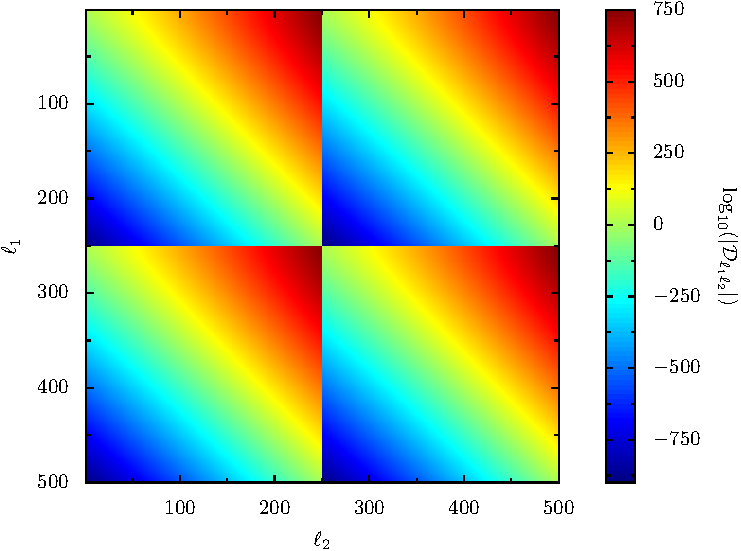
\includegraphics[scale=0.95]{plots/numeric/matrix/matrix1.pdf}
    \subcaption{$T=0.1$, $n=1$, $m=1$}
    \end{minipage}
    \ \\
    \begin{minipage}[b]{\linewidth}
    \centering
    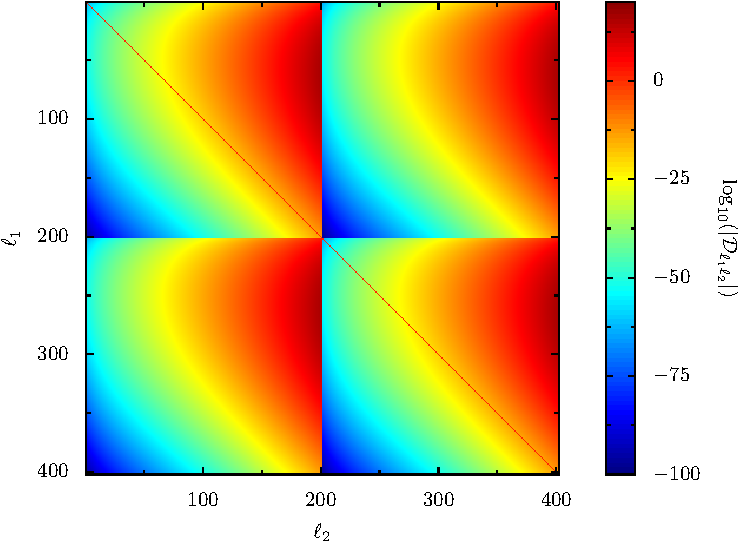
\includegraphics[scale=0.95]{plots/numeric/matrix/matrix2.pdf}
    \subcaption{$T=5$, $n=50$, $m=50$}
    \end{minipage}

  \caption{Two scattering matrices for $L/R=0.02$ and different values of $T$, $n$ and $m$. The matrix elements
  in a) differ by more than thousand orders of magnitude, in b)
  by more than hundred orders of magnitude.
  In a) the Matsubara frequency is $\xi_1=0.1$
  and the matrix elements scale similar to the $\xi\to0$ case. For this reason, the condition
  of the matrix can be improved by multiplying each matrix element with a factor $(nTR/\mathcal{L})^{\ell_2-\ell_1}$
  (cf. section \ref{section_scattering_ps_xi0}, in particular eqs. \eqref{scattering_ps_xi0_EE} and \eqref{scattering_ps_xi0_MM}).
  The structure of matrix b) is more complicated and no simple transformation that improves the condition is known.
  The red line on the diagonal in b) corresponds to the identity matrix, $\mathcal{D}=\Id-\mathcal{M}$.
  }
  \label{fig:numerical_matrix_elements}
\end{figure}

Due to the Mie coefficients and the integrals, the matrix elements may become
very small or very large. This is a very challenging numerical problem for two
reasons: The matrix elements must be computed and stored, and the algorithm
that calculates the determinant must handle an ill-conditioned matrix whose
entries differ by hundreds of orders of magnitude. Fig. \ref{fig:numerical_matrix_elements}
shows two examples of ill-conditioned matrices.

Modern computers use the IEEE 754 standard \cite{IEEE:1985:AIS} for floating
point computations. The standard defines arithmetic formats with single
(32 bits) and double precision (64 bits). A double can represent
numbers in the range from $4.94\cdot10^{-324}$ to $1.80\cdot10^{308}$. However,
this is not sufficient for small separations.
We present here three different solutions that all have been implemented
in the numerical program.


\subsection{Using logarithms}

The idea of this solution is to represent matrix elements by its logarithms.
This way we drastically expand the range of representable
numbers. In doing so, we also increase the holes between representable numbers.
However, numerical tests show that this raises no computational problems.

The logarithm of a negative number is complex. As we want to use real numbers,
we have to store the sign separately. So, we represent a number $a$ by
\begin{equation}
\tilde a = (-1)^{s_a} \log |a|,
\end{equation}
where $s_a = \text{sgn}(a)$.
A major drawback of this method is that we cannot use basic arithmetic
operations like addition or multiplication anymore. Multiplication
of two numbers $a$ and $b$ becomes trivial, as it becomes an addition
\begin{equation}
\widetilde{ab} = (-1)^{s_a+s_b} \left( \log|a| + \log|b|\right).
\end{equation}
The addition of two numbers is more complicated. We must take
care of the signs of both numbers and avoid over- and underflows:
\begin{equation}
\widetilde{(a+b)} =  \left\{
    \begin{array}{cl}
        (-1)^{s_b} \log \, |b|,                                                                               & \mbox{if } \log \, |a| = -\infty \\ 
        (-1)^{s_a} \log \, |a|,                                                                               & \mbox{if } \log \, |b| = -\infty \\ 
        (-1)^{s_a} \left[\log \, |a| + \log{\left(1+(-1)^{s_a+s_b}\e^{\log \, |b|-\log \, |a|}\right)}\right], & \mbox{if } \log \, |a| > \log \, |b| \\ 
        (-1)^{s_b} \left[\log \, |b| + \log{\left(1+(-1)^{s_a+s_b}\e^{\log \, |a|-\log \, |b|}\right)}\right], & \mbox{otherwise}
    \end{array}
\right.
\end{equation}
Many programming languages provide a function $\text{log1p}(x)$ that returns
the natural logarithm of 1+x in a way which is accurate for small values of $x$.

This method only depends on double arithmetics. Double arithmetics is fast and
supported on almost every platform. But additions
become costly, as they usually involve the computation of the exponential and
the logarithm function. Besides, the code becomes obfuscated.


\subsection{Quadruple precision}

Another way to solve the problem is the use of 128 bits quadruple precision.
Quadruple precision is supported by the GNU C Compiler (gcc) and the Intel C
Compiler (icc). Quads have an exponent of 15 bits and cover almost 9900 orders
of magnitude. However, usually processors do not support quads and the
operations have to be carried out in software which makes quad arithmetics very
slow.  The increase of computational time renders this method impractical for
actual calculations, yet it is a good way to estimate the numerical stability
of the two faster methods.


\subsection{Extended double precision}

On x86 and x86-64 processors the floating point unit (FPU) supports the extended
precision format with 80 bits and 15 bits exponent. The extended double format
covers the same range of numbers like quadruple precision, is more precise than
the double format, but less precise than the quaduple format. Gcc and icc
support the extended double format and also provide a library with basic mathematical
functions. The actual calculations are performed in the floating point unit.
Extensions to the x86 instruction set like SSE only support the double
format and thus the compiler cannot use these extensions for optimizations and
parallelizations. However, this is still the fastest solution. It is about a
factor of 10 faster than quads and a factor of 2 faster than the logarithm
approach.


\subsection{Conclusion}

\begin{table}
\begin{center}
\begin{tabular}{|l|l|l|l|}
\hline
            & logarithm approach   & extended double precision     & quadruple precision \\
\hline
runtime     & $\approx2$x          & 1x                            & $\approx10$x \\
\hline
accuracy    & ok                   & good                          & excellent \\
\hline
portability & almost all platforms & most compilers on x86, x86-64 & few compilers \\
\hline
readability & poor                 & good                          & good \\
\hline
\end{tabular}
\caption{Comparison of the three different solutions. The runtime is
given compared to the runtime using the extended double format.}
\label{tab:numerics_melements_conclusion}
\end{center}
\end{table}

All calculations in this master thesis are carried out using extended double precision
unless otherwise stated. This is the fastest method with a good accuracy and in
most cases the best choice. On non x86 or x86-64 platforms the logarithm
approach still gives good results, but it is about a factor of 2 slower. The
quadruple precision is only useful when comparing results with one of the other
methods, in all other cases quadruple precision is too slow for actual
computations. The three approaches are compared in table
\ref{tab:numerics_melements_conclusion}.


\section{Determinant}

The scattering matrix $\mathcal{D}$ is ill-conditioned and the calculation of
its determinant is sensitive to rounding errors. In order to improve the
accuracy, the matrix must be balanced before computing the determinant. The
balancing procedure uses similarity transformations to make corresponding rows
and columns have comparable norms, while leaving the determinant of the matrix
unchanged \cite{NumericalRecipesInFortran, HandbookOfAutomaticComputation}.
This is the key point of the calculation of the determinant: Without balancing, the
calculation of the determinant is numerically unstable.

After balancing, the determinant is calculated using a QR decomposition of the scattering matrix
into a product of an orthogonal matrix $Q$ and an upper triangle matrix $R$:
\begin{equation}
\mathcal{D} = QR
\end{equation}
The QR decomposition is computed with a series of Givens rotations
\cite{MatrixComputations}. After the QR decomposition, the logarithm of the
determinant of the scattering matrix can be computed easily:
\begin{equation}
\log \det \mathcal{D} =
\log \det R = \log \det \left(
\begin{array}{cccc}
a_{11} & a_{12} & a_{13} & \dots \\
       & a_{22} & a_{23} & \dots \\
       &        & a_{33} & \dots \\
0      &        &        & \ddots
\end{array}
\right) = \log \prod_{k=1}^N a_{kk} = \sum_{k=1}^N \log \, a_{kk}
\end{equation}

\section{Truncation of the infinite sum over $n$}
\label{numerics_truncation_sumn}

\begin{figure}
  \begin{minipage}[b]{.5\linewidth}
  \centering
  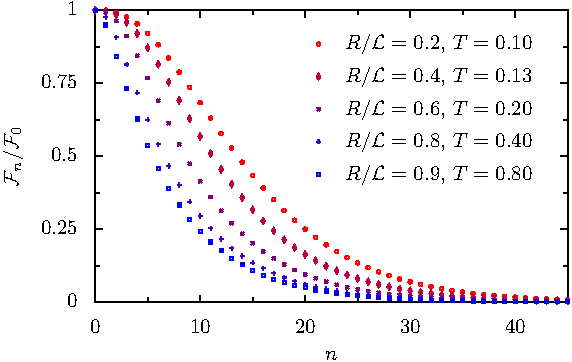
\includegraphics[scale=0.78]{plots/numeric/sumn/n.pdf}
  \subcaption{linear scale}
  \end{minipage}%
  \begin{minipage}[b]{.5\linewidth}
  \centering
  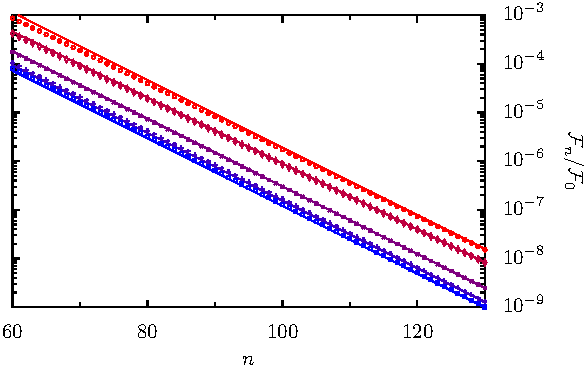
\includegraphics[scale=0.78]{plots/numeric/sumn/n_log.pdf}
  \subcaption{logarithmic scale}
  \end{minipage}

  \caption{Contributions of the $n$-th Matsubara frequency to the free energy:
  In a) we plot $\mathcal{F}_n/\mathcal{F}_0$ for different temperatures $T$ and
  aspect ratios $R/\mathcal{L}$. For $nT\gg1$ the contributions fall off exponentially.
  In b) we use a logarithmic scale for $\mathcal{F}_n/\mathcal{F}_0$. The symbols correspond to
  the same parameters as in plot a). 
  The solid lines correspond to $\mathcal{F}_n/\mathcal{F}_0 = \mathcal{F}_{130} \, \e^{-2nT\left(1-R/\mathcal{L}\right)}/\mathcal{F}_0$.}
  \label{fig:numeric_sumn}
\end{figure}

The free energy is given as an infinite sum over the Matsubara frequencies
$\xi_n=nT$ and every frequency $\xi_n$ yields an independent
contribution $\mathcal{F}_n$ to the free energy
\begin{equation}
\mathcal{F} = {\sum_{n=0}^\infty}^\prime \mathcal{F}_n.
\end{equation}
From a physical point of view it is obvious that this sum converges.
While the Mie coefficients grow exponentially for large Matsubara
frequencies $nT\gg1$ (cf. \eqref{eq:optical_properties_mie_large})
\begin{equation}
a_\ell \sim b_\ell \sim \e^{2nT \frac{R}{\mathcal{L}}},
\end{equation}
the integrals \eqref{scattering_int_A_scaled}--\eqref{scattering_int_D_scaled} decrease exponentially
\begin{equation}
A_{\ell_1,\ell_2,p}^{(m)} \sim B_{\ell_1,\ell_2,p}^{(m)} \sim C_{\ell_1,\ell_2,p}^{(m)} \sim D_{\ell_1,\ell_2,p}^{(m)} \sim \e^{-2nT}.
\end{equation}
In fact, the behaviour of the integrals is more complicated, however, for our
argumentation it is sufficient that they decrease somehow exponentially.
If we also assume that for $nT\gg1$ the matrix elements become small,
we can approximate the logarithm of the determinant of the scattering
matrix by a trace
\begin{equation}
\log \det \left(\Id - \mathcal{M}\right) \approx - \Tr \mathcal{M}.
\end{equation}
So we expect that the contributions to the free energy
$\mathcal{F}_n$ decrease like
\begin{equation}
\label{eq:numerics_sumn_exp}
\mathcal{F}_n \sim \exp{\left[-2nT\left(1-\frac{R}{\mathcal{L}}\right)\right]} \\ \text{for} \, \, nT \gg 1.
\end{equation}
Although our argumentation is oversimplifying, it is surprising that the result
is not too bad: Fig. \ref{fig:numeric_sumn} shows that the contributions to the
free energy decrease vaguely as predicted by \eqref{eq:numerics_sumn_exp}.

The numerical implementation cannot sum up infinite elements, but we have to
crop the sum at some point. Therefore, we split the series in a
finite sum that we compute and a remainder that we neglect:
\begin{equation}
{\sum_{n=0}^\infty}^\prime \mathcal{F}_n = {\sum_{n=0}^k}^\prime \mathcal{F}_n + R_k.
\end{equation}
We determine the value of $k$ using the inequality
\begin{equation}
\frac{\mathcal{F}_k}{\mathcal{F}_0} \le \epsilon_p, \\ \text{where} \, \, \epsilon_p \in (0,1).
\end{equation}
Smaller values of $\epsilon_p$ yield better accuracies.
The remainder may be estimated using \eqref{eq:numerics_sumn_exp}:
\begin{equation}
\label{eq:numerics_sumn_remainder}
R_k = \sum_{n=k+1}^\infty \mathcal{F}_n \simeq 
\mathcal{F}_k \sum_{n=1}^\infty q^n = \mathcal{F}_k \frac{q}{1-q}, \\ q = \e^{-2T\left(1-\frac{R}{\mathcal{L}}\right)}
\end{equation}
Eq. \eqref{eq:numerics_sumn_remainder} can be used to increase the accuracy for
a given value of $\epsilon_p$. However, the implementation does not use this
estimation yet.


\section{Truncation of the sum over $m$}

\begin{figure}
  \begin{minipage}[b]{.5\linewidth}
  \centering
  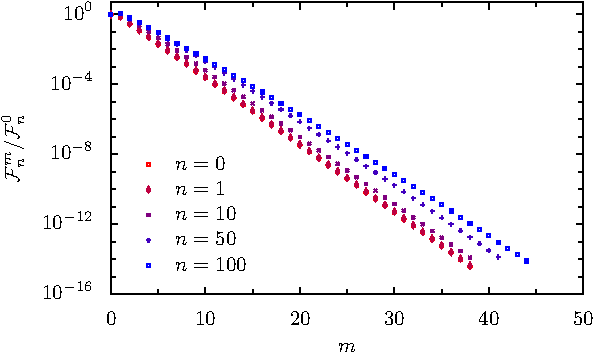
\includegraphics[scale=0.77]{plots/numeric/summ/RbyL0_1_T0_5.pdf}
  \subcaption{$L/R = 0.1$, $T=0.5$}
  \end{minipage}%
  \begin{minipage}[b]{.5\linewidth}
  \centering
  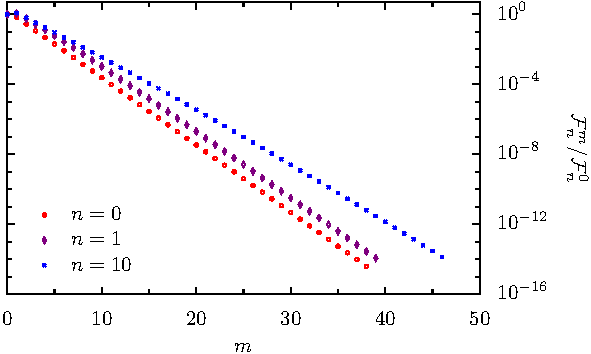
\includegraphics[scale=0.77]{plots/numeric/summ/RbyL0_1_T10_0.pdf}
  \subcaption{$L/R = 0.1$, $T=10$}
  \end{minipage} \\
  \ \\
  \begin{minipage}[b]{.5\linewidth}
  \centering
  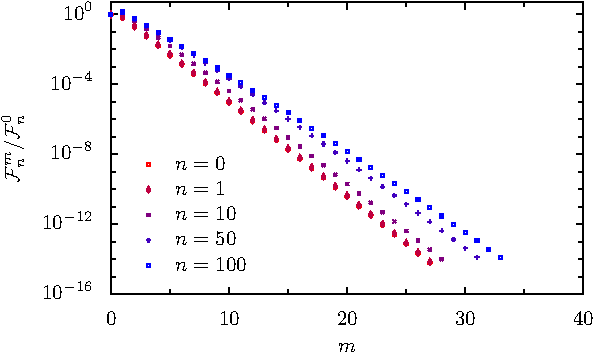
\includegraphics[scale=0.77]{plots/numeric/summ/RbyL0_2_T0_5.pdf}
  \subcaption{$L/R = 0.2$, $T=0.5$}
  \end{minipage}
  \begin{minipage}[b]{.5\linewidth}
  \centering
  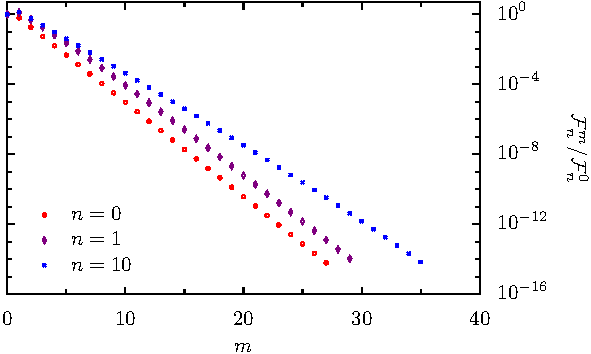
\includegraphics[scale=0.77]{plots/numeric/summ/RbyL0_2_T10_0.pdf}
  \subcaption{$L/R = 0.2$, $T=10$}
  \end{minipage}

  \caption{Decrease of the contributions to the free energy dependent on $m$ for fixed values of $n$.}
  \label{fig:numerics_summ}
\end{figure}

After the truncation of the vector space, the sum over $m$ is finite
\begin{equation}
\mathcal{F}_n = \sum_{m=0}^\lmax \mathcal{F}^m_n
\end{equation}
and all terms can be computed. Fig. \ref{fig:numerics_summ} shows the contributions
to $\mathcal{F}_n$ dependent on $m$ for different temperatures and separations. The
contributions to the free energy fall off exponentially. This means that terms for
high values of $m$ are extremely slight and can be neglected. This improves the
run-time of the numerics as less terms have to be computed. The summation is
aborted when
\begin{equation}
\frac{\mathcal{F}_n^k}{\sum_{m=0}^k \mathcal{F}^m_n} \le \epsilon_p,
\end{equation}
where $\epsilon_p$ is as in section \ref{numerics_truncation_sumn}. As
the contributions decrease exponentially, the remainder $R_k$ may be estimated
by
\begin{equation}
R_k = \sum_{m=k+1}^\lmax \mathcal{F}^m_n \approx \mathcal{F}_n^k \sum_{m=1}^{\lmax-k} q^k,
\end{equation}
where $q$ can be obtained by linear regression. Although this would increase the
accuracy of the result, the implementation does not support this feature yet.


\section{Numerical differentiation}

The force and the entropy are given as derivatives of the Casimir free energy
\begin{equation}
F = -\frac{\partial\mathcal{F}}{\partial L}, \\
S = -\frac{\partial\mathcal{F}}{\partial T}.
\end{equation}
In order to calculate the derivative of a function $f(x)$ we use the
finite difference formula of order 4 \cite{Fornberg88}
\begin{equation}
f^\prime(x) = \frac{-f(x+2h)+8f(x+h)-8f(x-h)+f(x-2h)}{12h} + \frac{h^4}{30}f^{(5)}(c),
\end{equation}
where $c\in [x-2h, x+2h]$. A detailed discussion about problems and errors of
numerical differentiation can be found in \cite{NumericalRecipesInFortran}.


\section{Numerical stability}

The accuracy of the result depends on the choices of $\lmax$ and $\epsilon_p$
as well as on round-off and other numerical errors. The first kind of errors,
i.e. the dependence of the accuracy on $\lmax$ and $\epsilon_p$, was investigated in
previous sections. In this section, we want to investigate the numerical
stability of the program. Under stability we unterstand the stability of the
program for fixed parameters. In simple words, we ask: ``Does the result change
if we calculate with higher precision while keeping the values of $\lmax$ and
$\epsilon_p$ fixed?''

Most numerical results of this master thesis have been computed using extended double
format. However, the numerical program also supports the more accurate quad
format. The extended double format gives about 18 significant decimal digits
while the quad format gives about 33. This way we can compare the
results of both implementations. The program is believed to be reliable if
both implementations yield (almost) same results. ``Almost same results'' means
that the deviation of both implementations
\begin{equation}
\Delta = \left| \frac{\mathcal{F}^\text{extended double}\left(T, \frac{L}{R}\right) - \mathcal{F}^\text{quad}\left(T, \frac{L}{R}\right)}{\mathcal{F}^\text{quad}\left(T, \frac{L}{R}\right)} \right|
\end{equation}
is not larger than the estimated numerical error due to the truncation of the
scattering matrix, and the truncations of the sums over $n$ and $m$.

\begin{figure}
    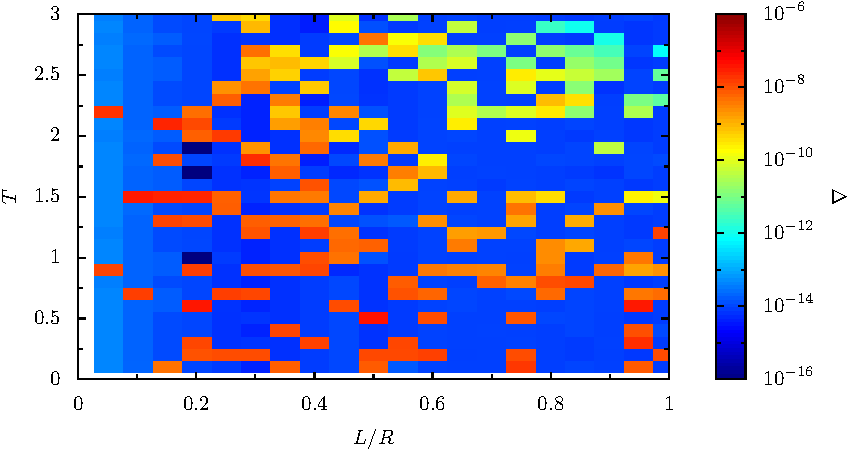
\includegraphics[scale=1]{plots/numeric/stability/stability.pdf}

    \caption{Deviations of the free energy calculated using extended double and quad format. Both
    computations yield almost same results.}
    \label{fig:numerics_stability}
\end{figure}

In Fig. \ref{fig:numerics_stability} we plot the deviations of the results
obtained using extended double and quad format. We have used
$\lmax=\text{max}\left(20, \lceil\eta R/L\rceil\right)$ with $\eta=6$ and
$\epsilon_p = 10^{-7}$. The error due to $\lmax$ and $\epsilon_p$ is believed
to be about $10^{-4}$ to $10^{-5}$. We see that the deviations are smaller than
the accuracy.

The resolution of Fig. \ref{fig:numerics_stability} is 30 points for $T$ and 20
points for $L/R$. This is the reason why the points look like bricks. The
numerical results were obtained using parallelization. The parallelized
algorithm is non-deterministic, because the conditions for the truncation of
the sums over $m$ and $n$ may be checked too late and more terms than
neccessary have been computed. So, the non-deterministic algorithm is the main
reason for the ``noise'' in Fig. \ref{fig:numerics_stability}.


%\section{Tests}
%
%As we have seen the implementation of the Casimir effect in the plane--sphere geometry
%comes along with a lot of problems. This makes the code prone to errors. In order to
%detect and avoid errors unit tests and a revision control system were used:
%\begin{itemize}
%\item The unit tests test different functions of the code and compare the
%results with expected values. The tests cover the prefactors
%$\Lambda_{\ell_1\ell_2}^{(m)}$ and $\Xi_{\ell_1\ell_2}^{(m)}$, the Bessel
%functions $I_\nu$ and $K_\nu$, the Mie coefficients $a_\ell$ and $b_\ell$ and the
%integration.
%\item Git was used as a revision control system and it helped more than once to
%find errors in the development.
%\end{itemize}
